\chapter{Ingesta de los datos en el lago de datos}

Los datos que se van a analizar en este trabajo han sido proporcionados por el profesor en el archivo \texttt{datos_practica.tar.gz}. El primer paso es descomprimir el archivo y ver qué contiene. Para ello, se ejecuta el siguiente comando en la terminal:

\begin{lstlisting}[language=bash]
tar -xvzf datos_practica.tar.gz
\end{lstlisting}

Ahora desde la consola de Spark iremos cargando los datos en el lago de datos.

\section{Countries}

Los datos sobre los paises en el archivo \texttt{countries.txt} está en un formato no estándar: \texttt{name::<name> \#\# iso_code::<iso_code> \#\# dafif_code::<dafif_code>}, por lo que se va a tener que tratar como datos desectructurados (RDDs) y realizar una serie de trnsformaciones con el objetivo de realizar una limpieza de los datos y darle una estructura \texttt{name: string, iso_code: string,
dafif_code: string} para obtener un DataFrame. Una vez obtenido el Dataframe, se debe utilizar el conector csv para guardar los datos en el path \texttt{/practica/countries/} de HDFS.

Primero introducimos nuestro archivo en un RDD y lo mostramos:

\begin{lstlisting}[language=scala]
val rdd = sc.textFile("/home/bigdata/practica/countries.txt")
rdd.take(5).foreach(println)
\end{lstlisting}

\begin{figure}[H]
    \centering
    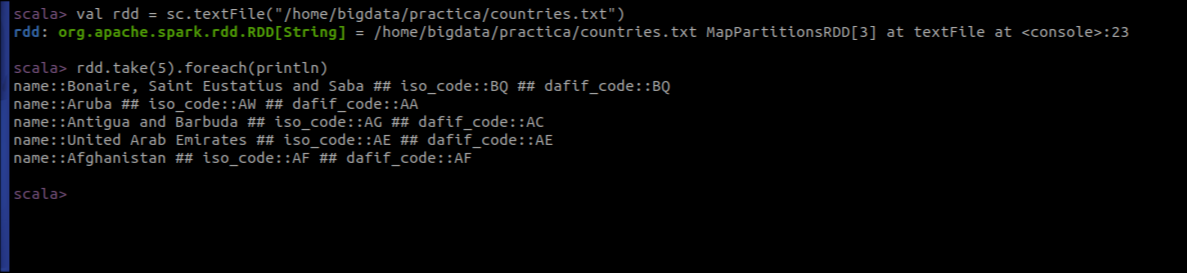
\includegraphics[width=0.8\textwidth]{figures/25.png}
    \caption{RDD de los países}
    \label{fig:countries_rdd}
\end{figure}

Ahora vamos a realizar una serie de transformaciones para limpiar los datos y darles una estructura. Para ello, vamos a utilizar el método \texttt{map} para dividir las líneas por el separador \texttt{##}, eliminar los espacios en blanco y eliminar los elementos vacíos. A continuación, filtramos las líneas que no tengan 3 elementos y mostramos el resultado:

\begin{lstlisting}[language=scala]
val lines = rdd.map(line => line.split("##").map(_.trim).filter(_.nonEmpty)).filter(_.size == 3)
lines.collect()(0)
\end{lstlisting}

\begin{figure}[H]
    \centering
    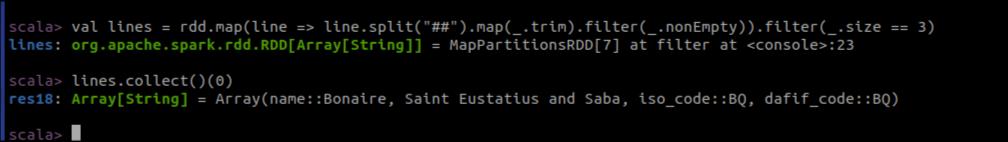
\includegraphics[width=0.8\textwidth]{figures/26.png}
    \caption{RDD de los países limpio}
    \label{fig:countries_rdd_clean}
\end{figure}

Crearemos la variable columnas en la que quitaremos el prefijo de las columnas (ej: \texttt{name::}) y mostraremos el resultado:

\begin{lstlisting}[language=scala]
val columns = lines.map(line => line.map(_.split("::")(1)))
columns.collect()(0)
\end{lstlisting}

\begin{figure}[H]
    \centering
    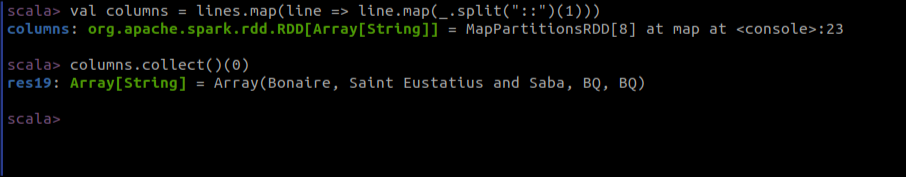
\includegraphics[width=0.8\textwidth]{figures/27.png}
    \caption{RDD de los países con nombres de columnas}
    \label{fig:countries_rdd_columns}
\end{figure}

Ahora ya si crearemos el dataframe de countries:

\begin{lstlisting}[language=scala]
val df_countries = columns.map(row => (row(0), row(1), row(2))).toDF("name", "iso_code", "dafif_code")
df_countries.show()
\end{lstlisting}

\begin{figure}[H]
    \centering
    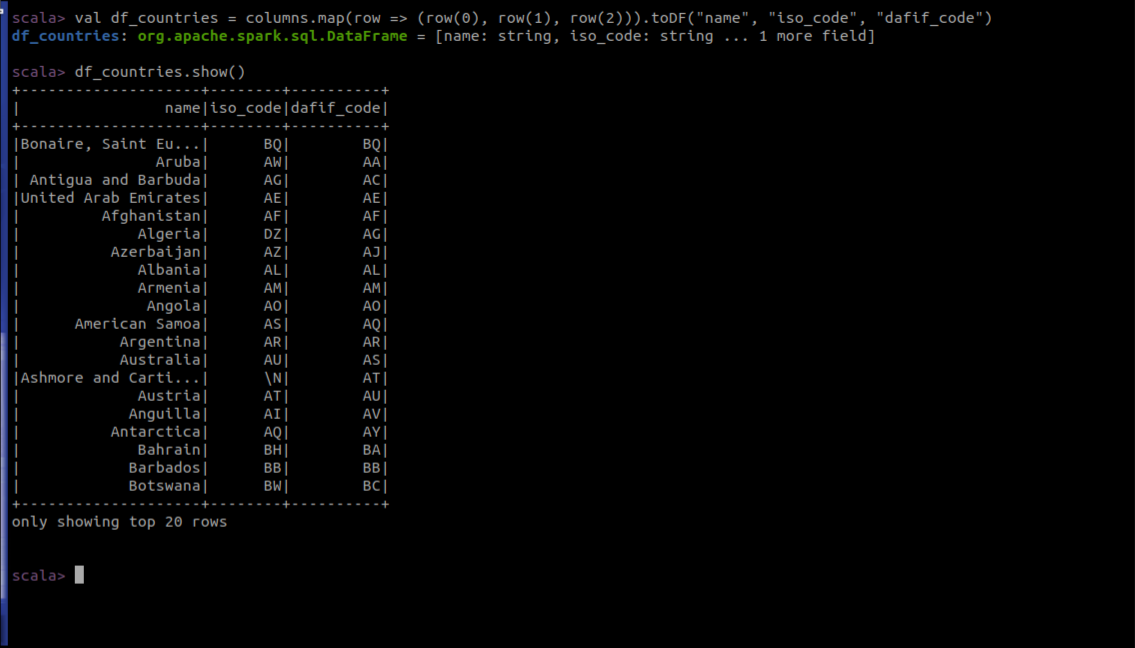
\includegraphics[width=0.8\textwidth]{figures/28.png}
    \caption{Dataframe de los países}
    \label{fig:countries_df}
\end{figure}

Ahora en otra terminal inciamos HDFS.

\begin{lstlisting}[language=bash]
hadoop-3.3.6/sbin/start-dfs.sh
\end{lstlisting}

\begin{figure}[H]
    \centering
    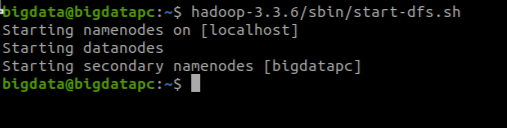
\includegraphics[width=0.8\textwidth]{figures/29.png}
    \caption{Iniciando HDFS}
    \label{fig:start_hdfs}
\end{figure}

Y guardamos el dataframe en HDFS desde la consola de scala:

\begin{lstlisting}[language=scala]
df_countries.write.format("csv").option("header","true").save("hdfs://localhost:9000/practica/countries/")
\end{lstlisting}

\begin{figure}[H]
    \centering
    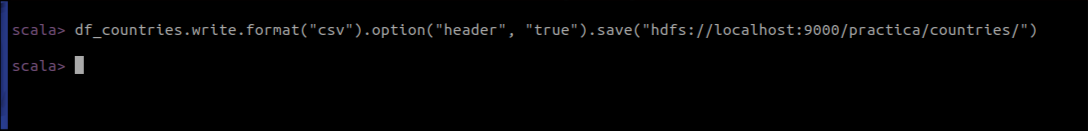
\includegraphics[width=0.8\textwidth]{figures/30.png}
    \caption{Guardando el dataframe en HDFS}
    \label{fig:save_df}
\end{figure}

Mostramos el contenido de la carpeta \texttt{/practica/countries/} en HDFS:

\begin{lstlisting}[language=bash]
hadoop-3.3.6/bin/hdfs dfs -ls /practica/countries/
\end{lstlisting}

\begin{figure}[H]
    \centering
    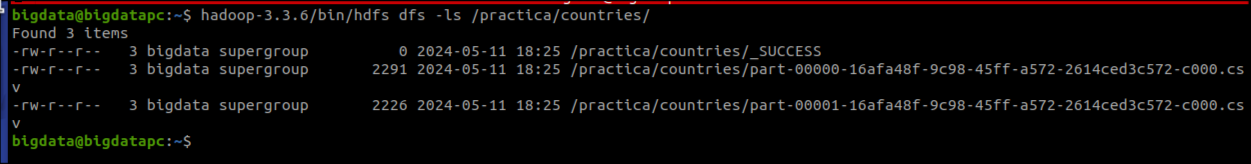
\includegraphics[width=0.8\textwidth]{figures/31.png}
    \caption{Contenido de la carpeta countries en HDFS}
    \label{fig:countries_hdfs}
\end{figure}

Por último, mostraremos 5 filas de los datos almacenados en HDFS:

\begin{lstlisting}[language=scala]
spark.read.format("csv").option("header", "true").option("inferSchema","true").load("hdfs://localhost:9000/practica/countries/").limit(5).show()
\end{lstlisting}

\begin{figure}[H]
    \centering
    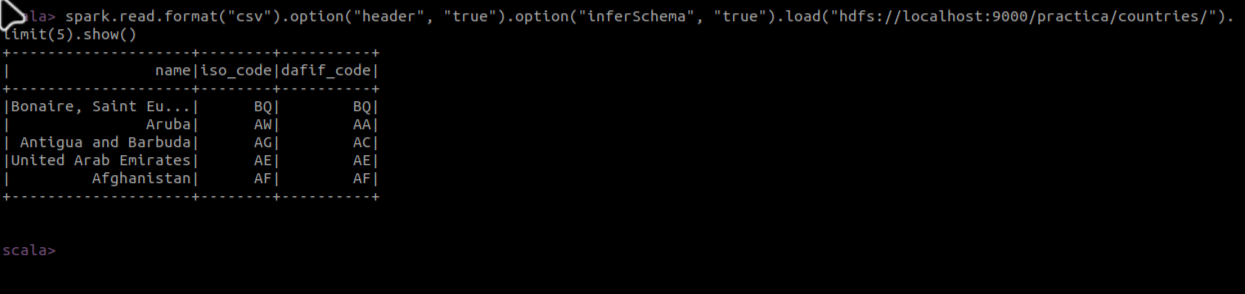
\includegraphics[width=0.8\textwidth]{figures/32.png}
    \caption{5 filas de los datos almacenados en HDFS}
    \label{fig:countries_hdfs_data}
\end{figure}

\section{Airlines}

Los datos sobre las aerolíneas están en el archivo \texttt{airlines.dat} y está en formato CSV. Por lo tanto, al ser datos estructurados, se puede cargar directamente en un DataFrame. Una de las columnas require una transformación ya que debería ser booleana en vez de string. Además, se nos pide añadir una columna nueva llamada \texttt{country_iso} que corresponde al \textit{iso_code} de los datos CSV que guardamos en HDFS. Una vez terminado, se debe utilizar el conector \textit{parquet} para guardar los datos particionados por la columna \textit{country} en el path \texttt{/practica/airlines/} de HDFS.

Primero cargamos los datos de airlines.dat en un Dataframe a través del conector de csv y las propiedades necesarias, para ello comenzaremos importando algunas estructuras de datos:

\begin{lstlisting}[language=scala]
import org.apache.spark.sql.types.StructType
import org.apache.spark.sql.types.StructField
import org.apache.spark.sql.types.StringType
import org.apache.spark.sql.types.IntegerType
import org.apache.spark.sql.types.FloatType
\end{lstlisting}

\begin{figure}[H]
    \centering
    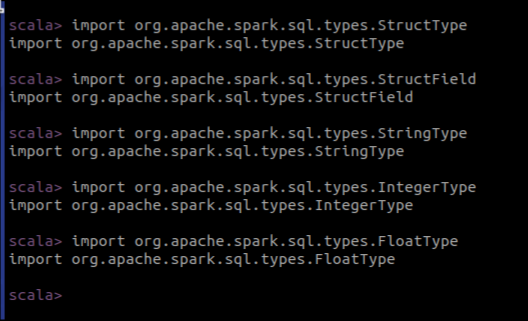
\includegraphics[width=0.8\textwidth]{figures/33.png}
    \caption{Importando estructuras de datos}
    \label{fig:import_data_structures}
\end{figure}

Después creamos un esquema para los datos de las aerolíneas:

\begin{lstlisting}[language=scala]
val airlines_schema = StructType(Array(StructField("id", IntegerType, true), StructField("name", StringType, true), StructField("alias", StringType,true), StructField("IATA", StringType, true),StructField("ICAO", StringType, true),StructField("callsign", StringType, true), StructField("country", StringType, true), StructField("active", StringType, true)))
\end{lstlisting}

\begin{figure}[H]
    \centering
    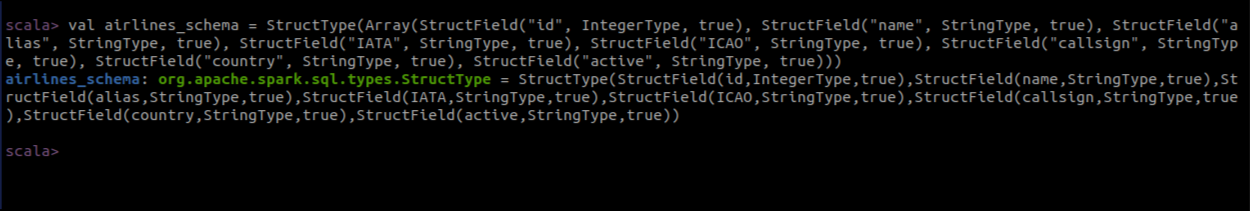
\includegraphics[width=0.8\textwidth]{figures/34.png}
    \caption{Creando el esquema de los datos de las aerolíneas}
    \label{fig:create_airlines_schema}
\end{figure}

Cargamos los datos en un DataFrame utilizando el esquema creado:

\begin{lstlisting}[language=scala]
var df_airlines = spark.read.format("csv").option("header", "false").schema(airlines_schema).load("/home/bigdata/practica/airlines.dat")
df_airlines.show()
\end{lstlisting}

\begin{figure}[H]
    \centering
    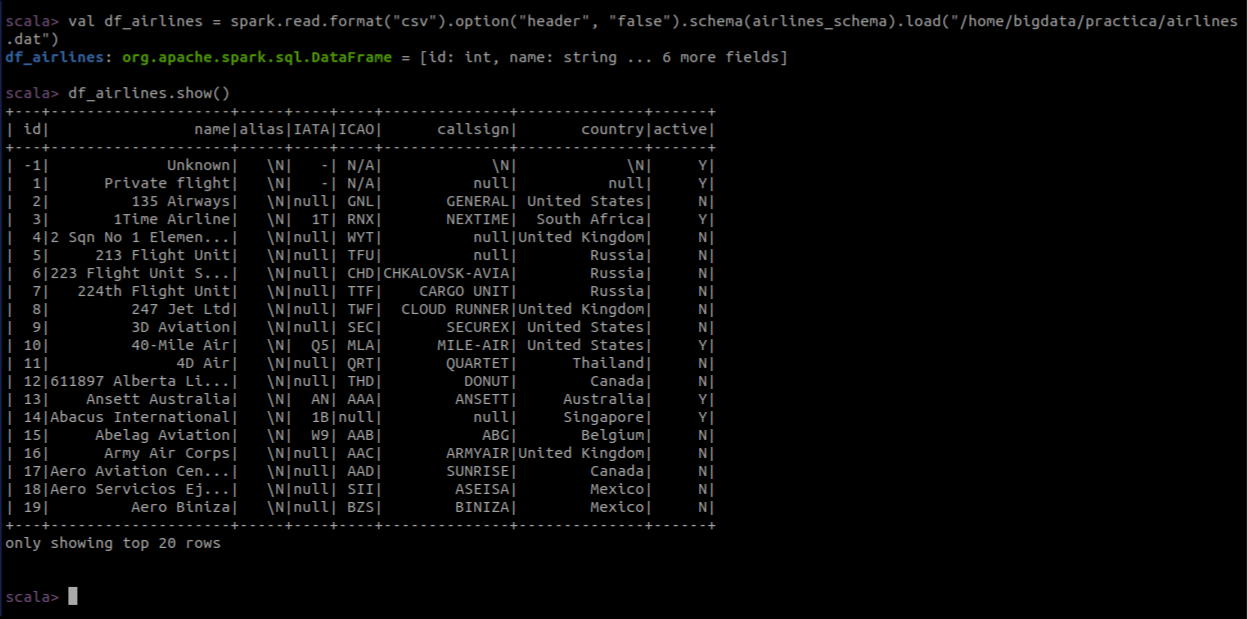
\includegraphics[width=0.8\textwidth]{figures/35.png}
    \caption{Dataframe de las aerolíneas}
    \label{fig:airlines_df}
\end{figure}

Ahora realizaremos las transformaciones necesarias para convertir los datos y el tipo de la columna active de String a Boolean

\begin{lstlisting}[language=scala]
    df_airlines = df_airlines.withColumn("active", when(col("active") === "Y", true).otherwise(false))
\end{lstlisting}

\begin{figure}[H]
    \centering
    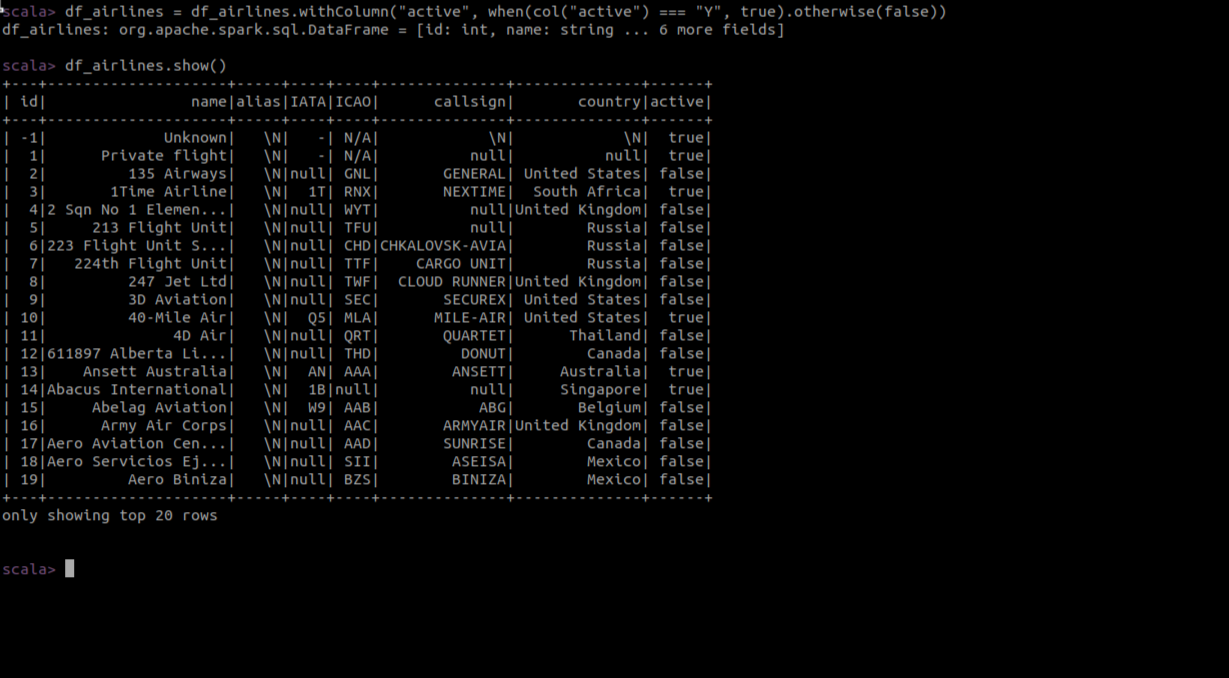
\includegraphics[width=0.8\textwidth]{figures/36.png}
    \caption{Dataframe de las aerolíneas con la columna active convertida a boolean}
    \label{fig:airlines_df_active}
\end{figure}

Ahora cargaremos los datos de los países en un DataFrame para poder unirlo con el DataFrame de las aerolíneas:

\begin{lstlisting}[language=scala]
var df_countries = spark.read.format("csv").option("header","true").option("inferSchema", "true").load("hdfs://localhost:9000/practica/countries/")
countries.show()
\end{lstlisting}

\begin{figure}[H]
    \centering
    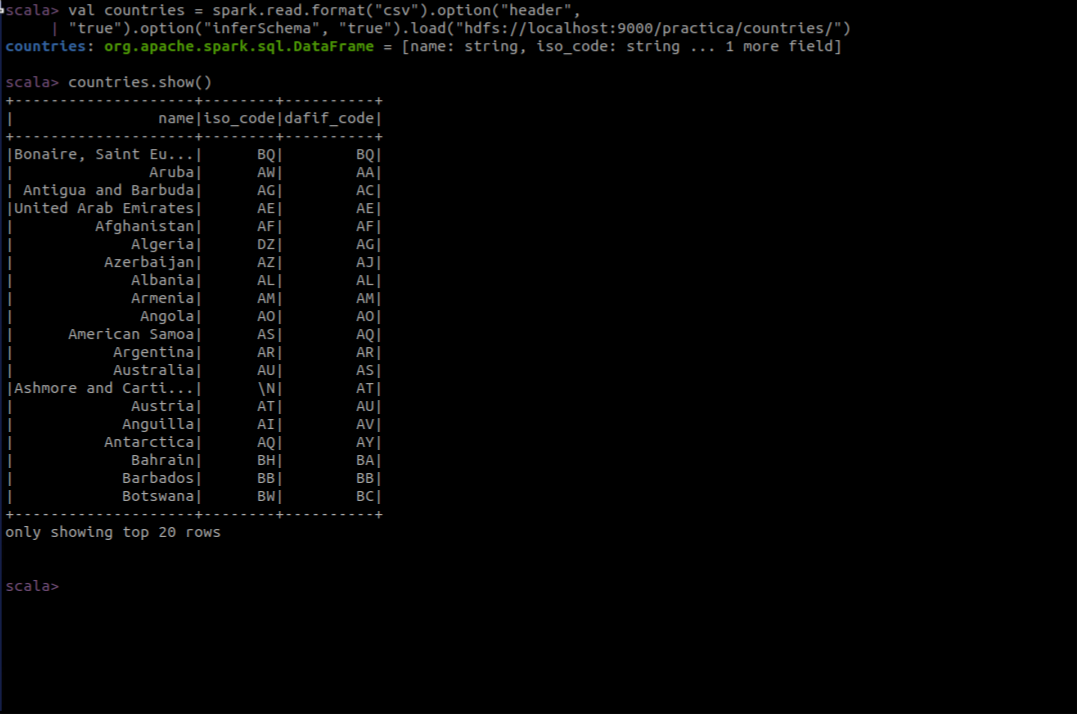
\includegraphics[width=0.8\textwidth]{figures/37.png}
    \caption{Dataframe de los países}
    \label{fig:countries_df_from_hdfs}
\end{figure}

Como \texttt{countries} y \texttt{df\_airlines} tienen una columna en común, \texttt{country}, tenemos que renombrar la columna \texttt{name} de countries a \texttt{country} para poder unir los dos DataFrames.

\begin{lstlisting}[language=scala]
df_countries = df_countries.withColumnRenamed("name", "country")
\end{lstlisting}

Ahora unimos los dos DataFrames por la columna \texttt{country} y renombramos la columna \texttt{iso_code} a \texttt{country_iso}:

\begin{lstlisting}[language=scala]
df_airlines = df_airlines.join(df_countries, Seq("country"), "left")
df_airlines = df_airlines.withColumnRenamed("iso_code", "country_iso")
\end{lstlisting}

\begin{figure}[H]
    \centering
    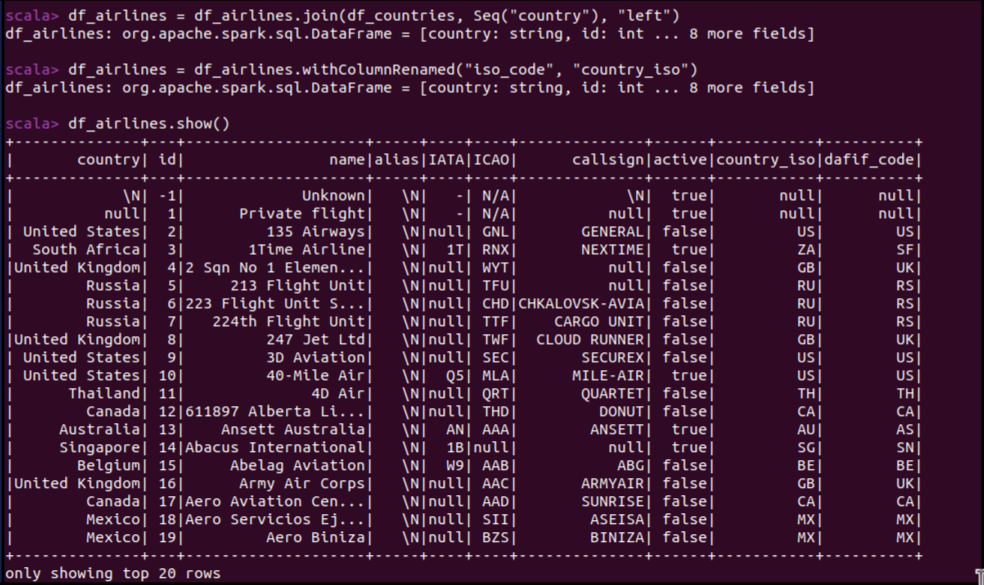
\includegraphics[width=0.8\textwidth]{figures/38.png}
    \caption{Dataframe de las aerolíneas con los países}
    \label{fig:airlines_countries_df}
\end{figure}

Vamos a eliminar la columna \texttt{darif_code} ya que no la necesitamos:

\begin{lstlisting}[language=scala]
df_airlines = df_airlines.drop("dafif_code")
\end{lstlisting}

También reordenaremos las columnas para que \texttt{id} sea la primera columna:

\begin{lstlisting}[language=scala]
df_airlines = df_airlines.select("id", "name", "alias", "IATA", "ICAO", "callsign", "country", "country_iso", "active")
\end{lstlisting}

\begin{figure}[H]
    \centering
    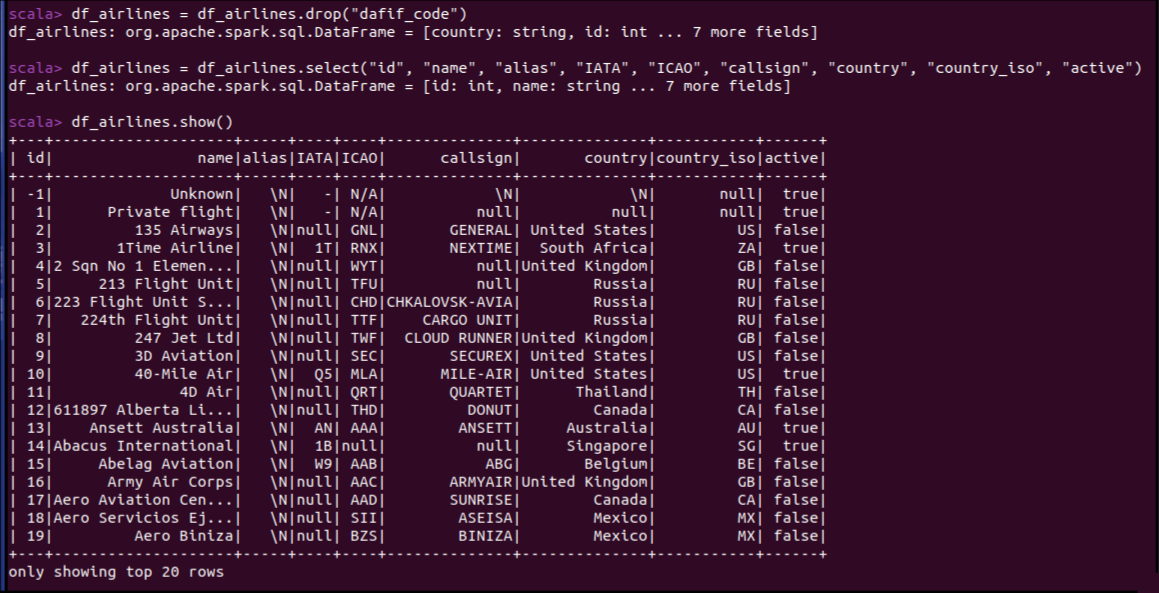
\includegraphics[width=0.8\textwidth]{figures/39.png}
    \caption{Dataframe de las aerolíneas con las columnas reordenadas}
    \label{fig:airlines_reordered_df}
\end{figure}

Vamos a eliminar las filas que tengan valores nulos o \texttt{\textbackslash N} en la columna \texttt{country}:

\begin{lstlisting}[language=scala]
df_airlines = df_airlines.filter(col("country").isNotNull && col("country") =!= "\\N"))
\end{lstlisting}

\begin{figure}[H]
    \centering
    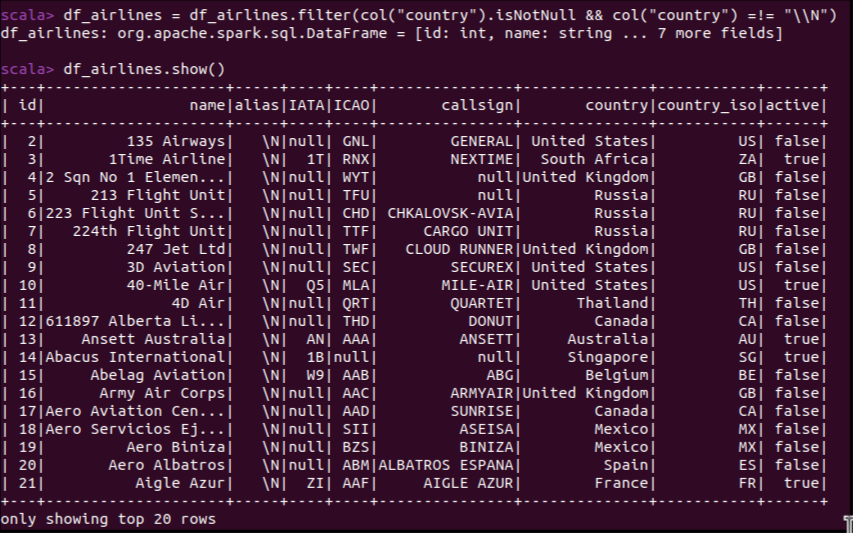
\includegraphics[width=0.8\textwidth]{figures/40.png}
    \caption{Dataframe de las aerolíneas sin valores nulos en la columna country}
    \label{fig:airlines_no_null_df}
\end{figure}

Por último, guardamos el DataFrame en HDFS particionado por la columna \texttt{country}:

\begin{lstlisting}[language=scala]
df_airlines.write.format("parquet").partitionBy("country").save("hdfs://localhost:9000/practica/airlines/")
\end{lstlisting}

Cargramos los datos de las aerolíneas desde HDFS y mostramos 5 filas:

\begin{lstlisting}[language=scala]
spark.read.format("parquet").load("hdfs://localhost:9000/practica/airlines/").limit(5).show()
\end{lstlisting}

\begin{figure}[H]
    \centering
    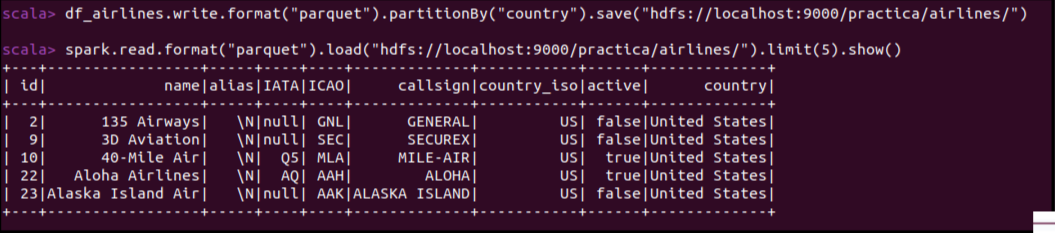
\includegraphics[width=0.8\textwidth]{figures/41.png}
    \caption{5 filas de los datos de las aerolíneas en HDFS}
    \label{fig:airlines_hdfs_data}
\end{figure}

\section{Airports}

Los datos sobre aeropuertos (fichero \texttt{airports.dat}) están en formato CSV. Por tanto, estos datos se pueden cargar en un Dataframe con el conector correspondiente y las opciones que se requieran. Una de las columnas está en una unidad de medida que no es compatible con los sistemas del cliente. Esa columna es \texttt{altitude} y sus valores están en pies. Para realizar la transformación a metros, se debe desarrollar una UDF y ser aplicada en dicha columna. Una vez obtenido este Dataframe, se debe utilizar el conector JDBC para guardar los datos en la tabla airports de Postgres. Además, el líder técnico de nuestro proyecto indica que, al hacer la lectura de estos datos, se deben añadir las propiedades \texttt{partitionColumn}, \texttt{lowerBound}, \texttt{upperBound} y \texttt{numPartitions} propias del conector JDBC.

Creamos el esquema de los datos de los aeropuertos:

\begin{lstlisting}[language=scala]
val airports_schema = StructType(Array(StructField("id", IntegerType, true), StructField("name", StringType, true), StructField("city", StringType, true), StructField("country", StringType, true), StructField("IATA", StringType, true), StructField("ICAO", StringType, true), StructField("latitude", FloatType, true), StructField("longitude", FloatType, true), StructField("altitude", IntegerType, true), StructField("timeZone", FloatType, true), StructField("DST", StringType, true), StructField("tz_database", StringType, true), StructField("tipo", StringType, true), StructField("source", StringType, true)))
\end{lstlisting}

\begin{figure}[H]
    \centering
    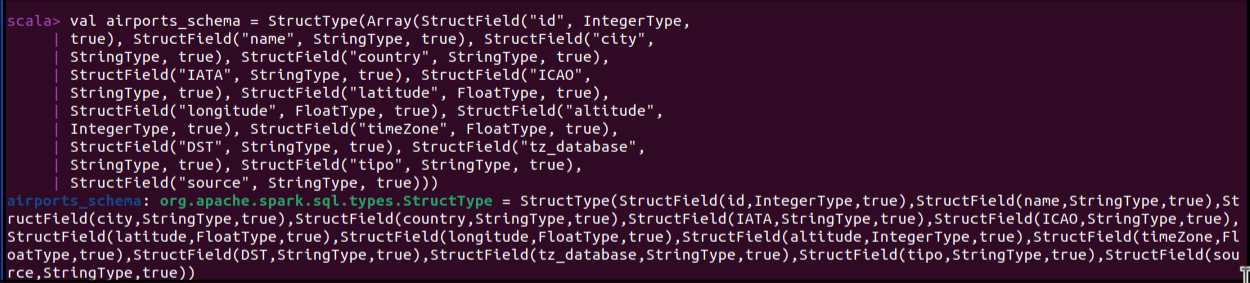
\includegraphics[width=0.8\textwidth]{figures/42.png}
    \caption{Creando el esquema de los datos de los aeropuertos}
    \label{fig:create_airports_schema}
\end{figure}

Cargamos los datos en un DataFrame utilizando el esquema creado:

\begin{lstlisting}[language=scala]
var df_airports = spark.read.format("csv").option("header", "false").schema(airports_schema).load("/home/bigdata/practica/airports.dat")
\end{lstlisting}

\begin{figure}[H]
    \centering
    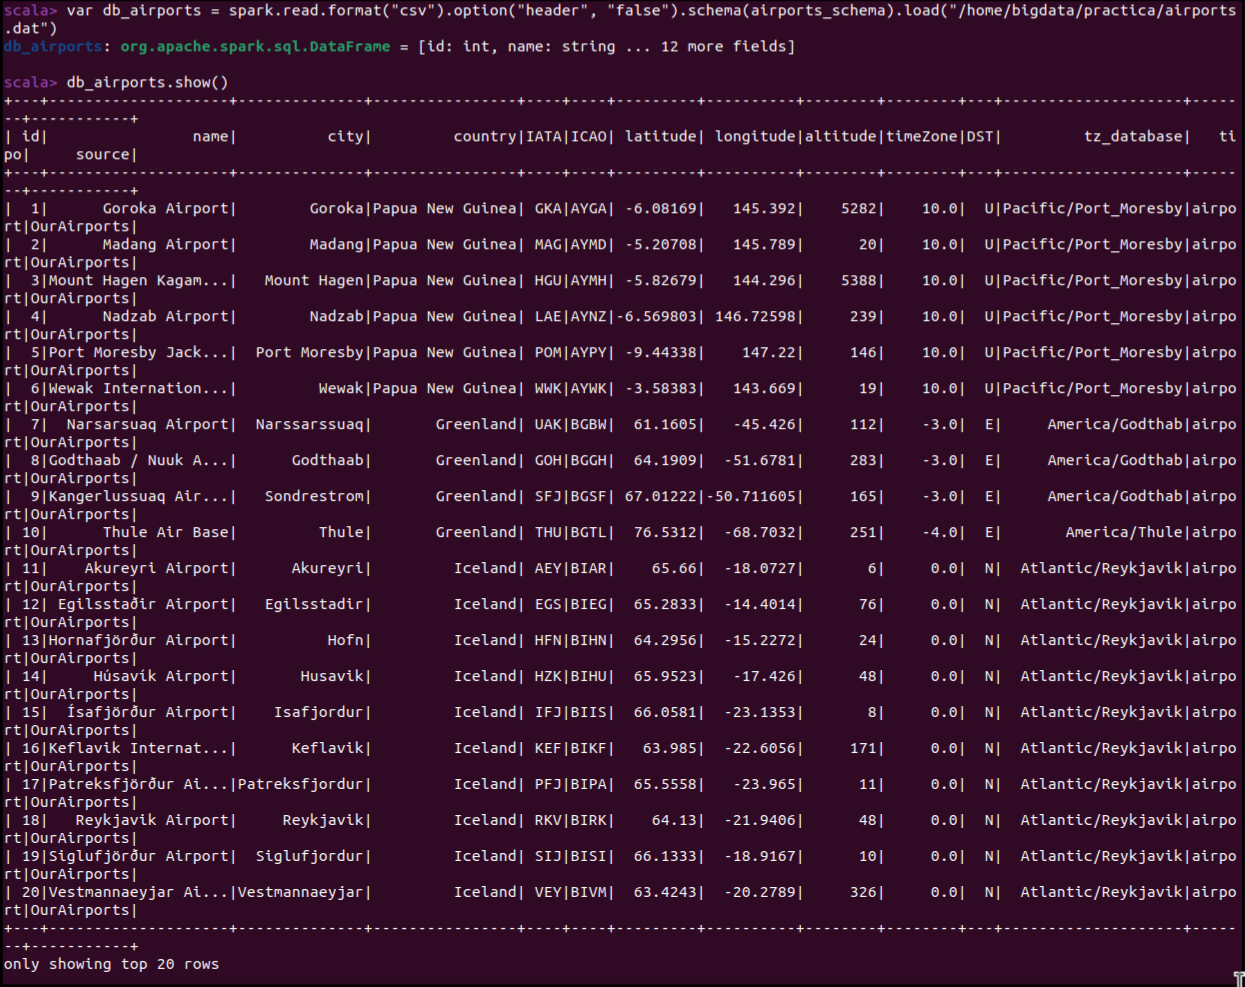
\includegraphics[width=0.8\textwidth]{figures/43.png}
    \caption{Dataframe de los aeropuertos}
    \label{fig:airports_df}
\end{figure}

Ahora haremos la conversión de la columna \texttt{altitude} de pies a metros, primero creamos la variable \texttt{feetToMeters} que será nuestra UDF:

\begin{lstlisting}[language=scala]
val feetToMeters = udf((x: Float) => x / 3.281)
\end{lstlisting}

\begin{figure}[H]
    \centering
    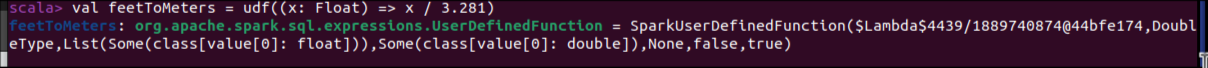
\includegraphics[width=0.8\textwidth]{figures/44.png}
    \caption{Creando la UDF feetToMeters}
    \label{fig:create_udf}
\end{figure}

Y aplicamos la UDF a la columna \texttt{altitude}:

\begin{lstlisting}[language=scala]
df_airports = df_airports.withColumn("altitude", feetToMeters(col("altitude")))
\end{lstlisting}

\begin{figure}[H]
    \centering
    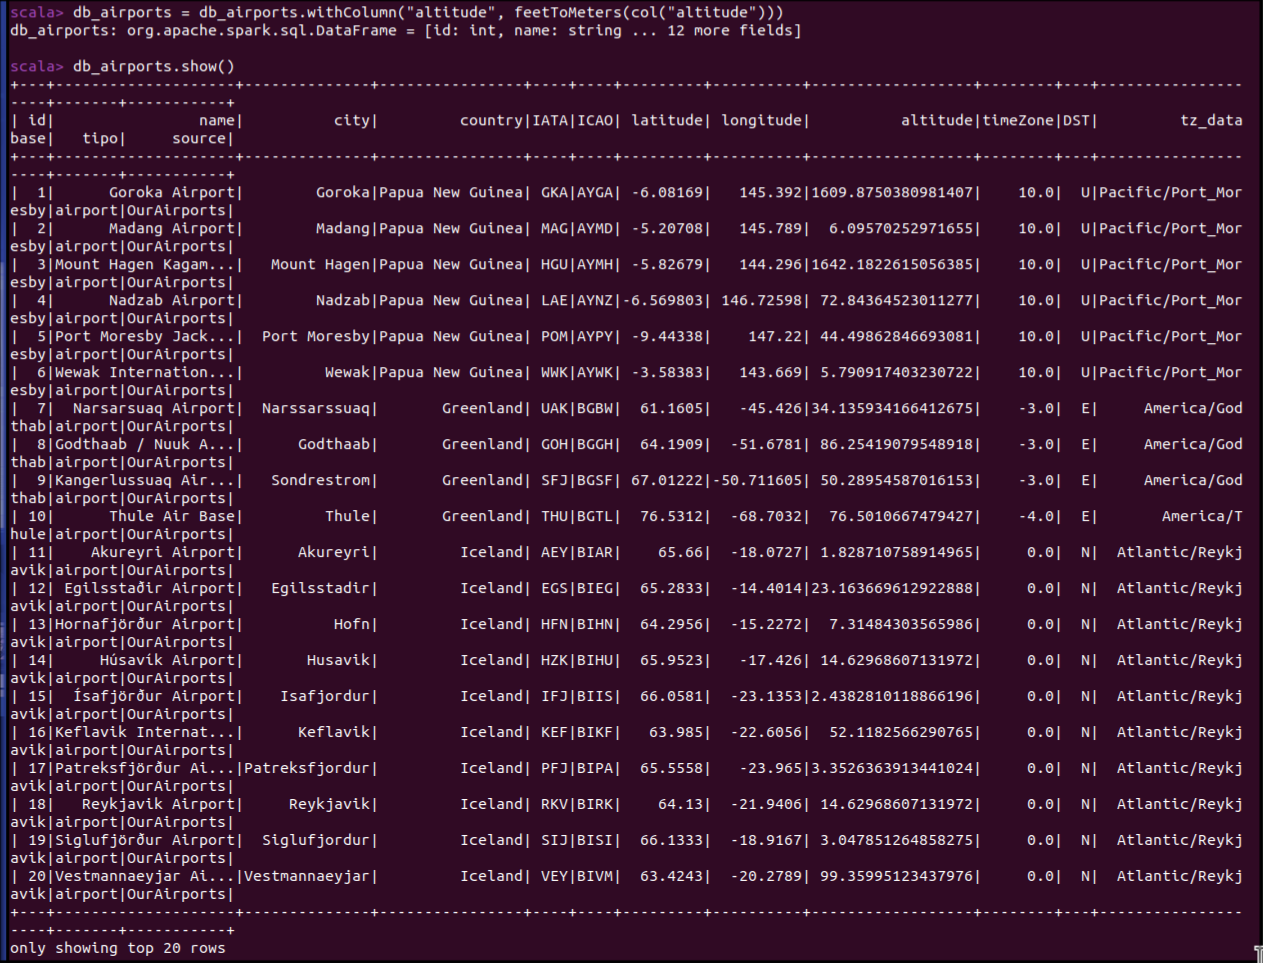
\includegraphics[width=0.8\textwidth]{figures/45.png}
    \caption{Dataframe de los aeropuertos con la columna altitude convertida a metros}
    \label{fig:airports_df_altitude}
\end{figure}

Para poder guardar los datos en la tabla \texttt{airports} de Postgres, primero la tendremos que crear. Primero nos metemos en la consola de Postgres:

\begin{lstlisting}[language=bash]
sudo -u postgres psql
\end{lstlisting}

\begin{figure}[H]
    \centering
    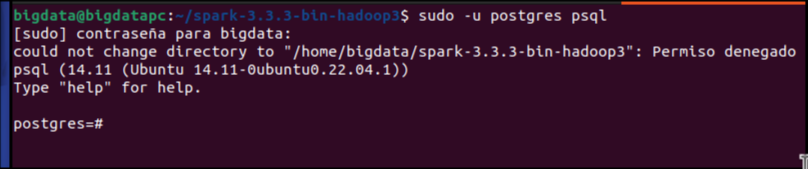
\includegraphics[width=0.8\textwidth]{figures/46.png}
    \caption{Entrando en la consola de Postgres}
    \label{fig:enter_postgres_console}
\end{figure}

Ahora creamos la tabla \texttt{airports}:

\begin{lstlisting}[language=sql]
CREATE TABLE airports(id INT, name VARCHAR(255), city VARCHAR(255), country VARCHAR(255), IATA VARCHAR(255), ICAO VARCHAR(255), latitude FLOAT, longitude FLOAT, altitude DOUBLE PRECISION, timeZone INT, DST VARCHAR(255), tz_database VARCHAR(255), tipo VARCHAR(255), source VARCHAR(255));
\end{lstlisting}

\begin{figure}[H]
    \centering
    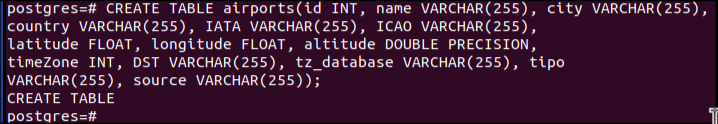
\includegraphics[width=0.8\textwidth]{figures/47.png}
    \caption{Creando la tabla airports en Postgres}
    \label{fig:create_airports_table}
\end{figure}

También deberemos darle una contraseña al usuario \texttt{postgres}:

\begin{lstlisting}[language=sql]
ALTER USER postgres WITH PASSWORD 'postgres';
\end{lstlisting}

\begin{figure}[H]
    \centering
    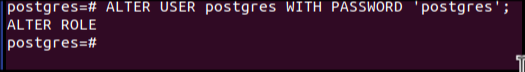
\includegraphics[width=0.8\textwidth]{figures/48.png}
    \caption{Dando una contraseña al usuario postgres}
    \label{fig:postgres_password}
\end{figure}

Guardamos los datos en la tabla \texttt{airports} de Postgres:

\begin{lstlisting}[language=scala]
import java.util.Properties
val properties = new Properties()

properties.setProperty("user", "postgres")
properties.setProperty("driver", "org.postgresql.Driver")
properties.setProperty("password", "postgres")
properties.setProperty("partitionColumn", "altitude")
properties.setProperty("lowerBound", "0")
properties.setProperty("upperBound", "2000")
properties.setProperty("numPartitions", "10")
properties.setProperty("password", "postgres")

df_airports.write.mode("overwrite").jdbc("jdbc:postgresql://localhost:5432/postgres", "airports", properties)
\end{lstlisting}

\begin{figure}[H]
    \centering
    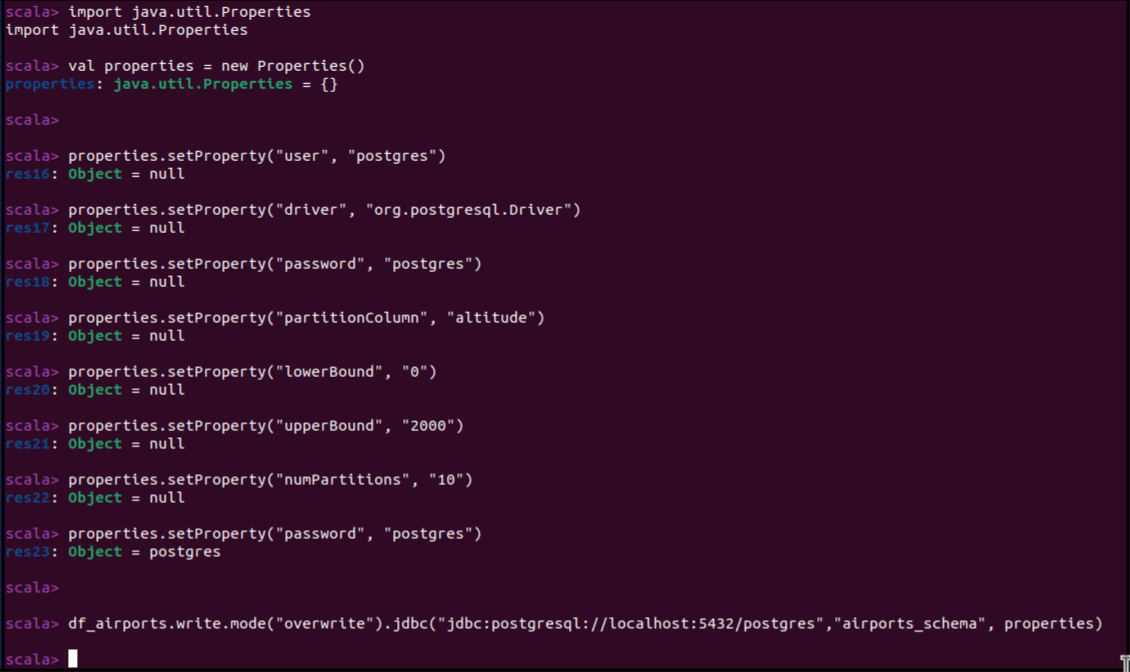
\includegraphics[width=0.8\textwidth]{figures/49.png}
    \caption{Guardando los datos en la tabla airports de Postgres}
    \label{fig:save_airports_postgres}
\end{figure}

Mostramos las 5 filas de la tabla \texttt{airports} de Postgres añadiendo los parámetros necesarios. Los parámetros \texttt{lowerBound} y \texttt{upperBound} se utilizan para definir el rango de valores de la columna \texttt{altitude} y \texttt{numPartitions} para definir el número de particiones. El parámetro \texttt{partitionColumn} se utiliza para definir la columna por la que se particionarán los datos. Es importante utilizar estos parámetros para mejorar el rendimiento de la lectura de los datos.

\begin{lstlisting}[language=scala]
spark.read.option("partitionColumn", "altitude").option("lowerBound", 0).option("upperBound", 2000).option("numPartitions", 10).jdbc("jdbc:postgresql://localhost:5432/postgres", "airports", properties).limit(5).show()
\end{lstlisting}

\begin{figure}[H]
    \centering
    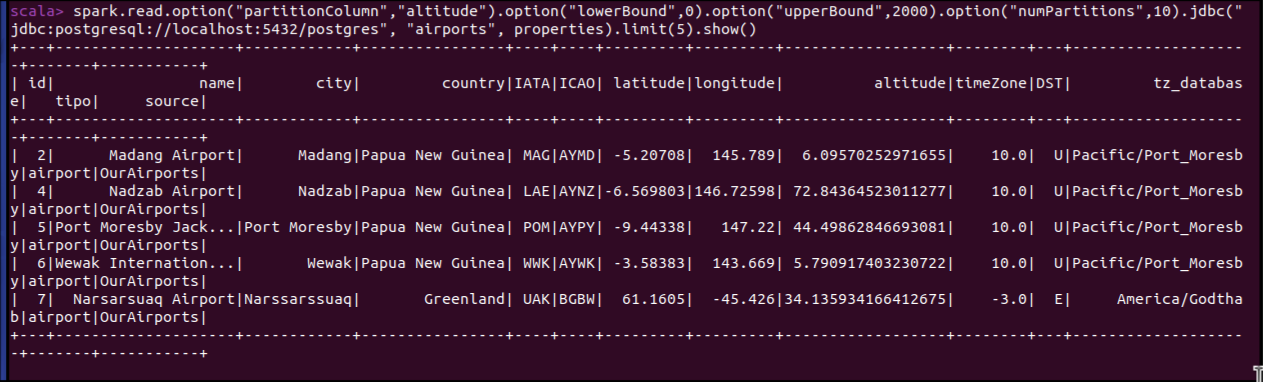
\includegraphics[width=0.8\textwidth]{figures/50.png}
    \caption{5 filas de la tabla airports de Postgres}
    \label{fig:airports_postgres_data}
\end{figure}

\section{Routes}

Antes de comenzar, es necesario utilizar un comando diferente para levantar la shell de spark. El JAR del conector de Cassandra no funciona correctamente, por lo que habrá que cargarlo mediante el paquete:

\begin{lstlisting}[language=bash]
bin/spark-shell --master spark://bigdatapc:7077 --executor-memory 2g --executor-cores 2 --jars jars/postgresql-42.7.3.jar  --packages com.datastax.spark:spark-cassandra-connector_2.12:3.3.0 --conf spark.cassandra.connection.host=localhost
\end{lstlisting}

Los datos sobre rutas (fichero \texttt{routes.dat}) están en formato CSV. Por tanto, estos datos se pueden cargar en un Dataframe con el conector correspondiente y las opciones que se requieran. Una vez obtenido este Dataframe, se debe utilizar el conector de Cassandra para guardar los datos en la tabla \texttt{routes} del keyspace practica.

Creamos el esquema de los datos de las rutas:

\begin{lstlisting}[language=scala]
val routes_schema = StructType(Array(StructField("airline", StringType, true), StructField("airline_id", IntegerType, true), StructField("source_airport", StringType, true), StructField("source_airport_id", IntegerType, true), StructField("destination_airport", StringType, true),StructField("destination_airport_id", IntegerType, true), StructField("codeshare", StringType, true), StructField("stops", IntegerType, true), StructField("equipment", StringType, true)))
\end{lstlisting}

\begin{figure}[H]
    \centering
    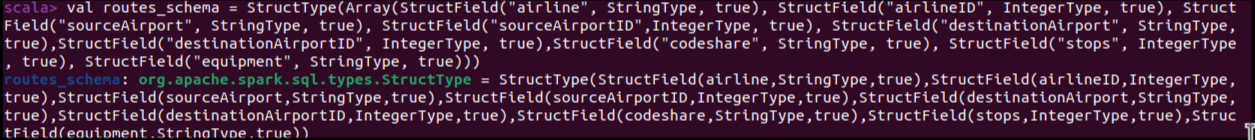
\includegraphics[width=0.8\textwidth]{figures/51.png}
    \caption{Creando el esquema de los datos de las rutas}
    \label{fig:create_routes_schema}
\end{figure}

Cargamos los datos en un DataFrame utilizando el esquema creado:

\begin{lstlisting}[language=scala]
val df_routes = spark.read.format("csv").option("header", "false").schema(routes_schema).load("/home/bigdata/practica/routes.dat")
\end{lstlisting}

\begin{figure}[H]
    \centering
    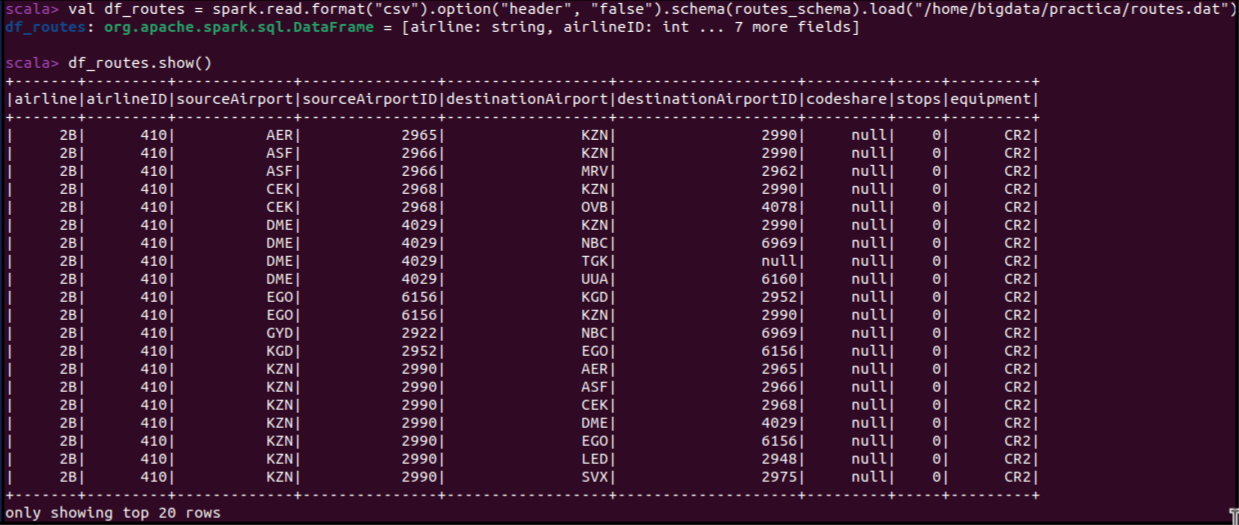
\includegraphics[width=0.8\textwidth]{figures/52.png}
    \caption{Dataframe de las rutas}
    \label{fig:routes_df}
\end{figure}

Vamos a añadir una columna \texttt{route_id} que será la primary key de la tabla \texttt{routes} de Cassandra. Para ello a cada fila le añadiremos un identificador único:

\begin{lstlisting}[language=scala]
import org.apache.spark.sql.functions.monotonically_increasing_id
df_routes = df_routes.withColumn("route_id", monotonically_increasing_id())
\end{lstlisting}

Reordenamos para que la columna \texttt{route_id} sea la primera:

\begin{lstlisting}[language=scala]
df_routes = df_routes.select("route_id", "airline", "airline_id", "source_airport", "source_airport_id", "destination_airport", "destination_airport_id", "codeshare", "stops", "equipment")
\end{lstlisting}

\begin{figure}[H]
    \centering
    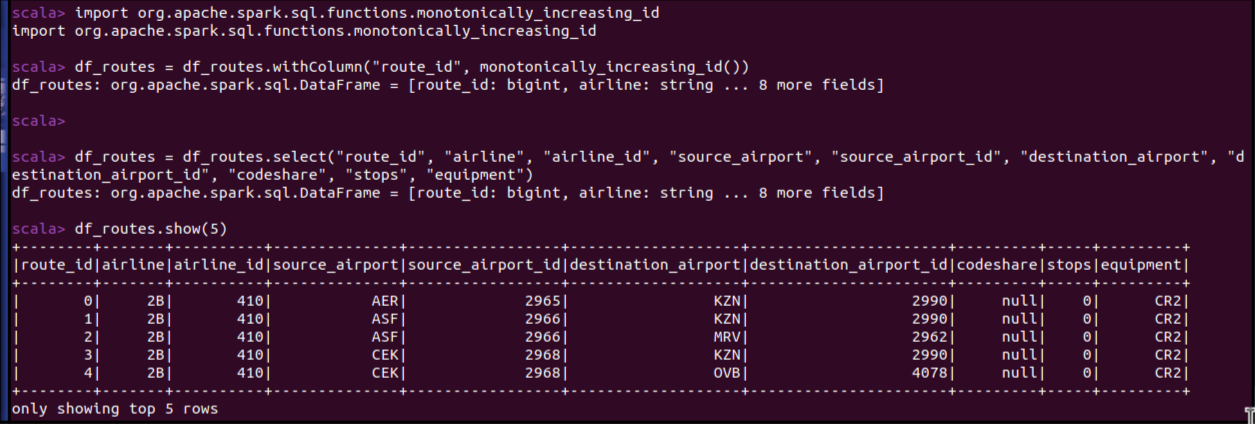
\includegraphics[width=0.8\textwidth]{figures/53.png}
    \caption{Dataframe de las rutas con la columna route\_id}
    \label{fig:routes_df_route_id}
\end{figure}

Creamos una nueva terminal y ejecutamos el siguiente comando para contectarnos a la shell de Cassandra:

\begin{lstlisting}[language=bash]
~/apache-cassandra-3.11.16/bin/cqlsh
\end{lstlisting}

\begin{figure}[H]
    \centering
    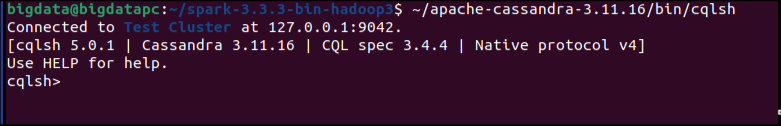
\includegraphics[width=0.8\textwidth]{figures/54.png}
    \caption{Entrando en la shell de Cassandra}
    \label{fig:enter_cassandra_shell}
\end{figure}

Creamos la tabla \texttt{routes} en el keyspace \texttt{practica}:

\begin{lstlisting}[language=sql]
USE practica;

CREATE TABLE routes (
    route_id int,
    airline text,
    airline_id int,
    source_airport text,
    source_airport_id int,
    destination_airport text,
    destination_airport_id int,
    codeshare text,
    stops int,
    equipment text,
    PRIMARY KEY (route_id)
);
\end{lstlisting}

\begin{figure}[H]
    \centering
    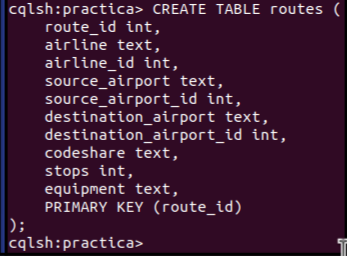
\includegraphics[width=0.8\textwidth]{figures/55.png}
    \caption{Creando la tabla routes en Cassandra}
    \label{fig:create_routes_table}
\end{figure}

Ahora ya podemos guardar los datos en la tabla \texttt{routes} del keyspace \texttt{practica} de Cassandra:

\begin{lstlisting}[language=scala]
df_routes.write.format("org.apache.spark.sql.cassandra").option("spark.cassandra.connection.host", "127.0.0.1").option("spark.cassandra.connection.port", "9042").option("keyspace", "practica").option("table", "routes").option("ttl", "1000").mode("append").save()
\end{lstlisting}

\begin{figure}[H]
    \centering
    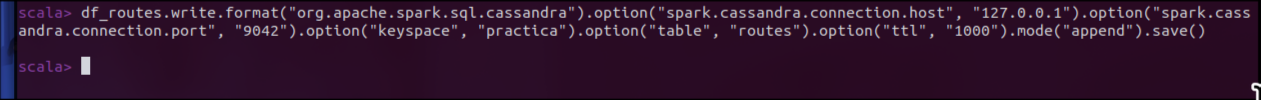
\includegraphics[width=0.8\textwidth]{figures/56.png}
    \caption{Guardando los datos en la tabla routes de Cassandra}
    \label{fig:save_routes_cassandra}
\end{figure}

Por último, mostraremos 5 filas de los datos en spark, almacenados en Cassandra:

\begin{lstlisting}[language=sql]
spark.read.format("org.apache.spark.sql.cassandra").option("spark.cassandra.connection.host", "127.0.0.1").option("spark.cassandra.connection.port", "9042").option("keyspace", "practica").option("table", "routes").load().limit(5).show()
\end{lstlisting}

\begin{figure}[H]
    \centering
    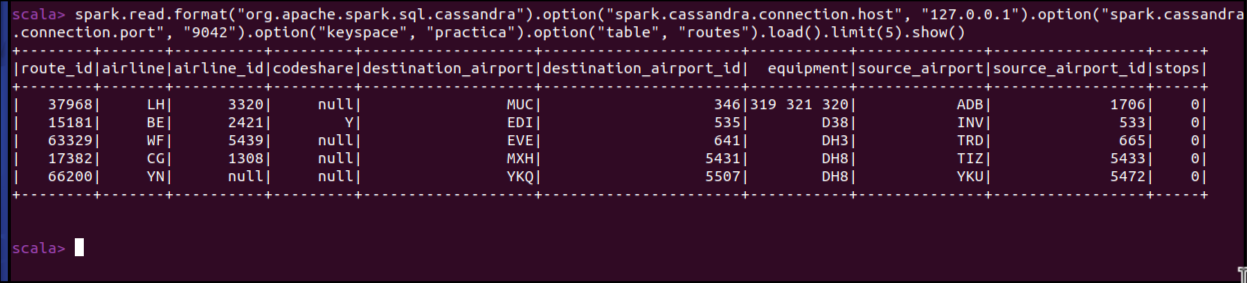
\includegraphics[width=0.8\textwidth]{figures/57.png}
    \caption{5 filas de los datos en la tabla routes de Cassandra}
    \label{fig:routes_cassandra_data}
\end{figure}
